%!TEX root = /Users/daniel/Documents/thesis/thesis.tex
\chapter{Motivation}

\section{\LaTeX}

Wenn es um das Verfassen wissenschaftlicher Texte geht, ist für viele \LaTeX\ die erste Wahl. Anders als bei einem \ac{WYSIWYG}-Editor kümmert man sich nicht um das Layout, um Abstände und Schriftgrößen sondern um die Semantik des Geschriebenen. Man zeichnet die Kapitel, Abschnitte, Formeln usw. aus, eher wie in \ac{HTML} als in MS-Word. Der Vorteil liegt auf der Hand. Inhalt und Präsentation sind klar getrennt, was zur Folge hat, dass man nicht vom Wesentlichen abgelenkt wird, wenn man an Texten und Formeln arbeitet, und dass das Aussehen des Dokuments zentral in der Präambel definiert wird.

\LaTeX~hat jedoch auch seine Nachteile. Gerade Anfänger haben es aufgrund der flachen Lernkurve schwer. Da man \LaTeX~in der Regel im Quelltext bearbeitet, also jeden Befehl von Hand schreibt, muss man sich unheimlich viel merken. Das beginnt bei einfachen Befehlen wie \texttt{\textbackslash chapter}, deren Name sich geradezu aufdrängt, aber wenn es darum geht Mathematische Formeln wie $$\Gamma \left( x \right) = \int\limits_0^\infty  {s^{x - 1} e^{ - s} ds}$$ in das Dokument zu bringen, wird es schon schwieriger.

Dass man ein $\Gamma$ mit dem Befehl \texttt{\textbackslash Gamma} bekommt ist noch zu erahnen. Um $\infty$ zu bekommen hätte man auch \texttt{\textbackslash infinity} statt \texttt{\textbackslash infty} versuchen können und hätte bloß einen Fehler geerntet, aber bei Befehlen wie \texttt{\textbackslash leftrightsquigarrow} ($\leftrightsquigarrow$) hört jede Intuition auf. Es ist also offensichtlich, dass es einigen Raum für unterstützende Maßnahmen bei der Erstellung von \LaTeX-Dokumenten gibt. Das gilt insbesondere für mathematische Formeln in denen viele unterschiedliche Symbole vorkommen können.

\section{Die optimale Eingabemethode}
\label{sec:optimal}

Überlegt man sich die natürlichste oder zumindest gewohnteste Art Text oder Mathematik zu notieren, so kommt man unweigerlich auf Stift und Papier. Während bei Texten die Eingabe über eine Computertastatur durchaus schneller sein kann als das Schreiben mit einem Stift, ist spätestens bei Formeln klar, dass hier der Stift seine Vorzüge hat\footnote{Allgemein ist die Eingabe mit einer Tastatur bei kleinen Alphabeten schneller, jedoch bei großen Alphabeten nicht mehr praktikabel \cite{Tappert:1990p10302}.}. Es können beliebige Formen, Zeichen und Symbole in beliebige räumliche Beziehung gebracht werden. Nichts liegt also näher, als diese Eingabeform in die digitale Welt übertragen zu wollen.

Als Eingabegerät bietet sich also ein Grafiktablett an. Ein entsprechender \LaTeX-Editor würde eine Fläche zur Verfügung stellen, auf die einfach geschrieben und skizziert wird. Die Kurven und Linien würden dann vom Editor in Text, Tabellen, Formeln und Diagramme überführt -- alles genau wie vom Benutzer erwartet. Dies ist eine Vision, die es seit 1995 gibt \cite{Meyer:1995p10480}. Leider sind wir 15 Jahre später immer noch nicht so weit.

Alleine der Bereich der mathematischen Formelerkennung ist noch nicht auf einem Level, auf dem man die verfügbaren Lösungen als gut bezeichnen könnte. Es gibt kaum kommerzielle Lösungen und eine Hand voll experimentelle Tools. Einige davon haben auch \LaTeX~oder Textsatz allgemein als Fokus. Andere gehen eher in Richtung interaktive Mathematik oder sogar \ac{CAS}.

\subsection[FFES]{FFES - Freehand Formula Entry System}
\label{sub:ffes}

\citet{Smithies:1999p11806} beschreiben ein weiteres System, mit dem Handgeschriebene Formeln in \LaTeX, Mathematica, oder eine LISP-artige Notation überführt werden können. Das System wird als Prototyp beschrieben. Leider habe ich das Projekt, dessen Quellcode frei verfügbar ist, nicht mehr zum Laufen bringen können und mir somit keinen eigenen Eindruck verschaffen können. Die Autoren gehen in ihrem Artikel die Problematik von Erkennungsfehlern unterschiedlicher Art ein und geben an, wie sie diese behandeln. Zum Beispiel stellen sie Gesten bereit, mit denen eine falsche Gruppierung von Strichen korrigiert werden kann. Symbolerkennungsfehler können mit Hilfe eines Kontextmenüs, das die wahrscheinlichsten $x$ Symbole anzeigt, korrigiert werden. Das größte Problem stellen den Autoren nach Fehler beim Parsen der Formel aufgrund von geringfügig deplatzierten Strichen dar, die durch manuelles Verschieben von Strichen korrigiert werden können. Hier besteht die Gefahr in eine frustrierende Formel-Debugging-Schleife zu geraten, da es häufig unklar ist, an welchem Strich der Algorithmus genau scheitert. Abbildung \ref{fig:ffes} zeigt das Benuzterinterface von FFES. Es ist der Internetseite \cite{ffes} entnommen, wo auch Quellcode erhältlich ist.

\begin{figure}
  \begin{center}
    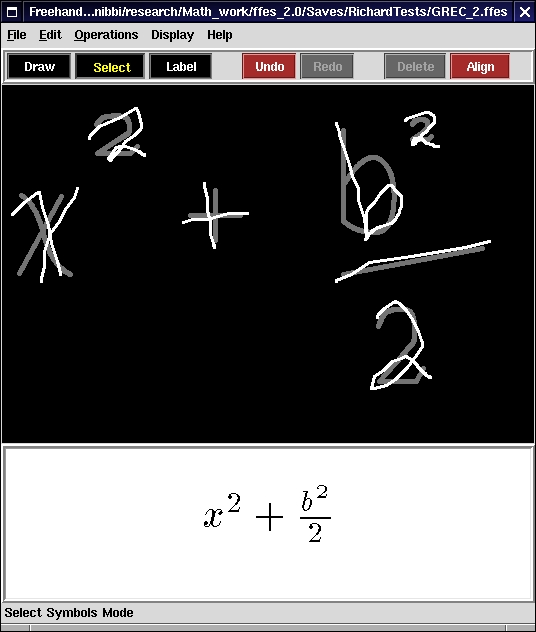
\includegraphics[width=.5\textwidth]{figures/ffes.png}
  \end{center}
  \caption{Freehand Formula Entry System}
  \label{fig:ffes}
\end{figure}

Die Autoren bemerken zudem, dass ihr System insbesondere für Experten nicht schneller zu bedienen ist, als klassische Systeme wie der Microsoft Equation Editor oder \LaTeX~aber es sei komfortabler und leichter zu lernen.

\subsection{Natural Log}
\label{sub:natural-log}

Natural Log ist von seinen Zielen her ähnlich wie FFES einzustufen. Das als Java-Applet implementierte Programm wandelt handgeschriebene Formeln und \LaTeX oder MathML um. Es kann unter \cite{natural-log} getestet werden. Als einzige Korrekturmöglichkeit bietet es die Möglichkeit Striche durch eine Geste wieder zu löschen. Leider ist Natural Log durch die fehlenden Korrekturmöglichkeiten überhaupt nicht zu gebrauchen. Die Verwendung ist eine Qual. Dem Autor \citet{Matasakis:1999p9465} ist dennoch Respekt geschuldet. Er hat sich nicht das leichteste Problem ausgesucht. Abbildung \ref{fig:natural-log} zeigt das Interface von Natural Log.

\begin{figure}
  \begin{center}
    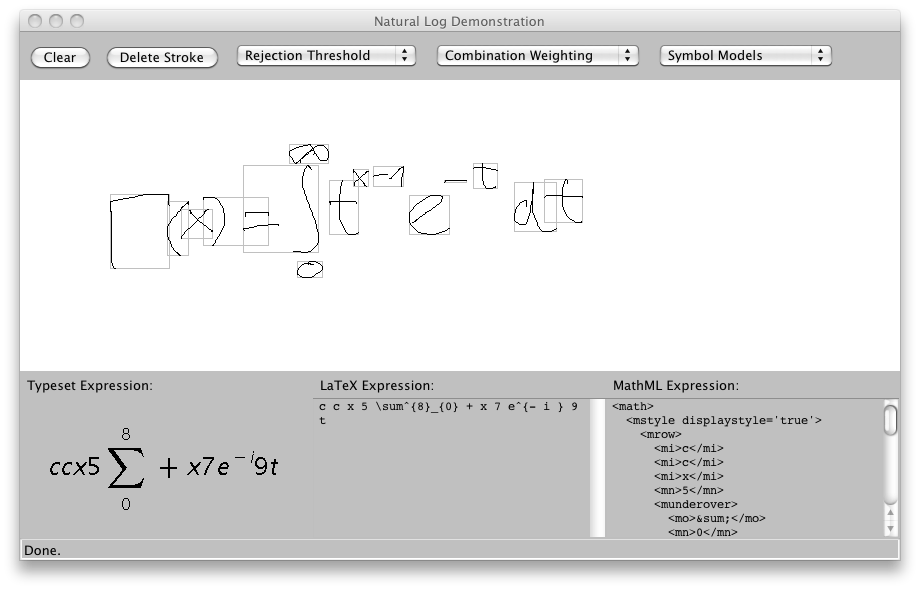
\includegraphics[width=.8\textwidth]{figures/natural-log.png}
  \end{center}
  \caption{Natural Log}
  \label{fig:natural-log}
\end{figure}

\subsection{JMathNotes}

JMathNotes ist ein weiteres Programm zur Konvertierung von handgeschriebenen Formeln in \LaTeX oder Mathematica.  Es ist wie Natural Log in Java implementiert, wird aber nicht als Applet zur Verfügung gestellt sondern es gibt für Linux und Windows Installationsprogramme. Es bietet dabei ähnliche Korrekturmöglichkeiten wie FFES. Die Gruppierung von Strichen kann korrigiert werden, einzelne Striche und ganze Symbole können verschoben werden und die Labels von falsch erkannten Symbolen können korrigiert werden. Für letzteres muss man allerdings das richtige Label kennen. Man bekommt nicht, wie in FFES beschrieben eine Auswahl der besten Treffer.
Im wesentlichen ist das JMathNotes von denselben Problemen geplagt, wie FFES obwohl es fünf Jahre später veröffentlicht wurde (FFES ist aus \citeyear{Matasakis:1999p9465} und JMathNotes aus \citeyear{jmathnotes}). Abbildung \ref{fig:jmathnotes} zeigt das Interface von JMathNotes.
%\cite{Tapia:2004p2713}

\begin{figure}
  \begin{center}
    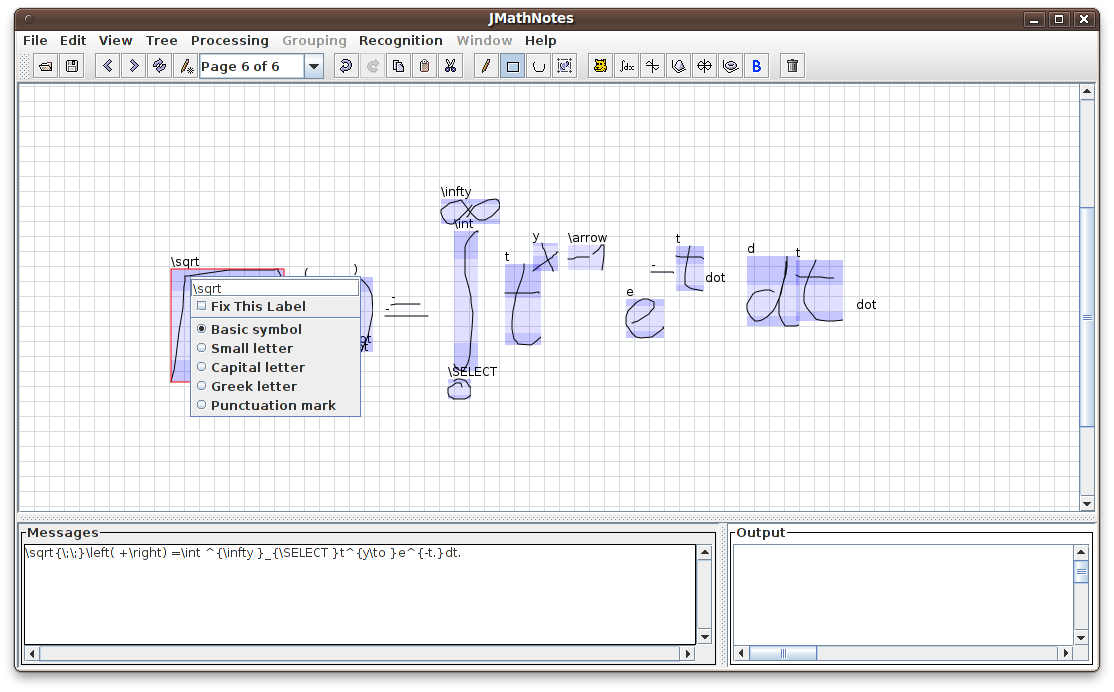
\includegraphics[width=\textwidth]{figures/jmathnotes.png}
  \end{center}
  \caption{JMathNotes}
  \label{fig:jmathnotes}
\end{figure}

\subsection{Infty Editor}

Ein weiteres Beispiel für einen Editor, der beim Textsatz helfen soll ist die kostenlose Software \href{http://www.inftyproject.org}{InftyEditor} \cite{Suzuki:2003p786}. Sie ermöglicht die Eingabe von Formeln in einem interessanten Mix aus \ac{WYSIWYG}-Editor und \LaTeX-Autovervollständigung mit Vorschau (siehe Abb.~\ref{fig:inftyeditor-autocomplete}). 

InftyEditor hat außerdem eine Funktion handgeschriebene Formeln zu erkennen. Dazu öffnet man das InftyHandWriting Input Pad und fängt an zu zeichnen. Die Erkennung erfolgt inkrementell also immer nach einem kurzen Zeitintervall nachdem der letzte Strich gezeichnet wurde. Die Korrekturmöglichkeiten beschränken sich darauf durch einen Klick auf Striche einige Möglichkeiten, wie diese zu interpretieren sind, durchzugehen. Einfache Formeln werden damit auch noch einigermaßen sicher erkannt, aber sobald die Komplexität der Formel steigt und vor allem sobald man Symbole braucht, die die Software gar nicht kennt, wird die Benutzung zum Frusterlebnis. Abb.~\ref{fig:inftyeditor} zeigt das InftyHandwriting Input Pad.

\begin{figure}
  \begin{center}
    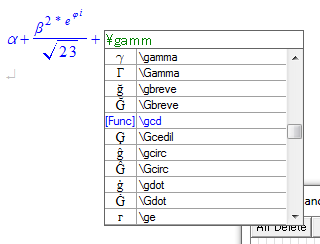
\includegraphics[width=.5\textwidth]{figures/inftyeditor-autocomplete.png}
  \end{center}
  \caption{InftyEditor Autovervollständigung}
  \label{fig:inftyeditor-autocomplete}
\end{figure}

\begin{figure}
  \begin{center}
    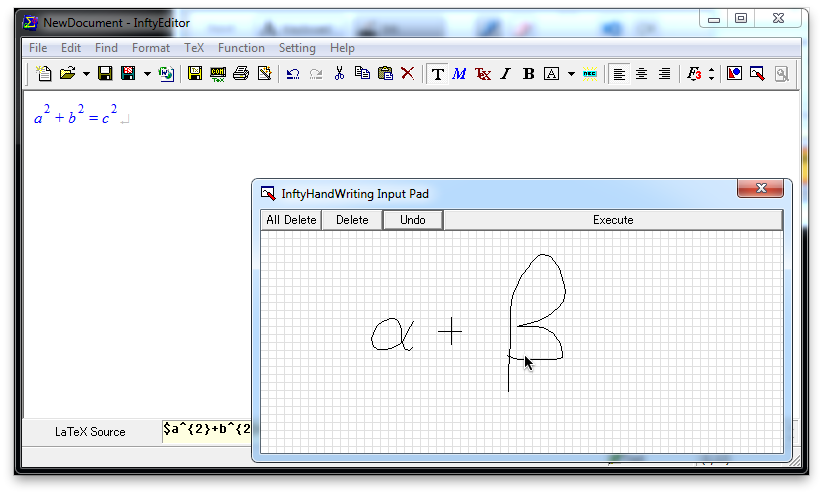
\includegraphics[width=.8\textwidth]{figures/inftyeditor.png}
  \end{center}
  \caption{InftyEditor}
  \label{fig:inftyeditor}
\end{figure}

\subsection{Microsoft Math}

Microsoft Math ist ein kommerzielles Produkt, das aber nicht für den Textsatz gedacht ist, sondern eher mit einem programmierbaren Taschenrechner zu vergleichen ist. Die Eingabe erfolgt entweder über die Tatstatur (Abb. \ref{fig:ms-math-keyboard}) oder über Handschrifterkennung (Abb. \ref{fig:ms-math-ink}) und die Handschrifterkennung macht zwar einen solideren Eindruck als bei den vorgenannten Produkten, ist aber auch noch nicht der Weisheit letzter Schluss. Abbildung \ref{fig:ms-math-ink} zeigt einen Versuch die Gammafunktion zu erkennen und der Erfolg ist zweifelhaft.

Ist die Formel dann auf welche Weise auch immer eingegeben, so kann dann damit einiges angestellt werden, was aber nicht im Interesse dieser Arbeit liegt und darum auch nicht näher beschrieben wird.

\begin{figure}
  \begin{center}
    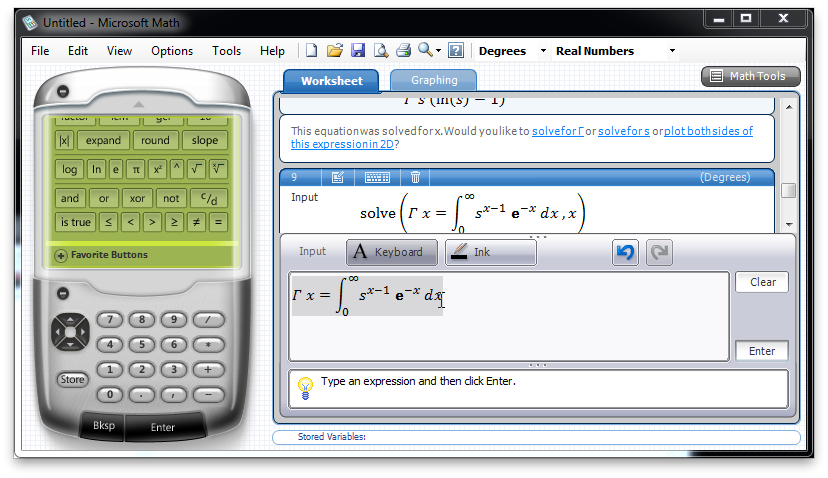
\includegraphics[width=.8\textwidth]{figures/ms-math-keyboard.png}
  \end{center}
  \caption{Microsoft Math 3.0 Tastatureingabe}
  \label{fig:ms-math-keyboard}
\end{figure}

\begin{figure}
  \begin{center}
    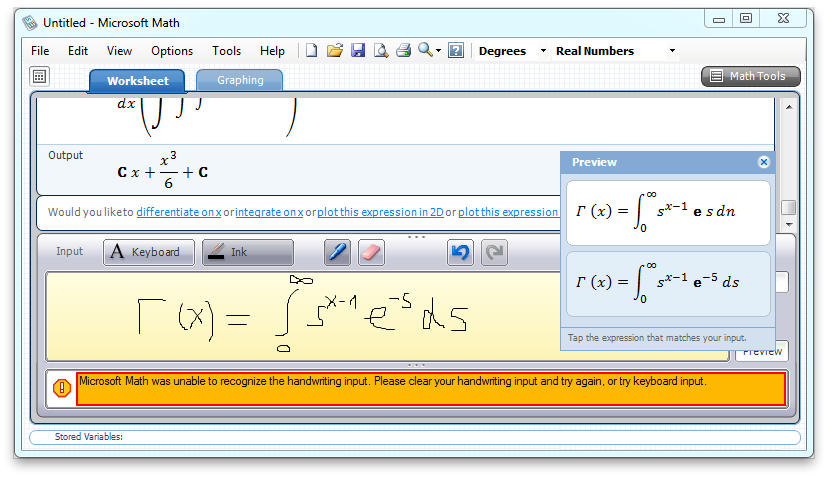
\includegraphics[width=.8\textwidth]{figures/ms-math-ink.png}
  \end{center}
  \caption{Microsoft Math 3.0 Handschrifterkennung}
  \label{fig:ms-math-ink}
\end{figure}


\subsection{MathJournal}

\citet{mathjournal} vertreibt eine weitere kommerzielle Software namens MathJournal. Sie ist an Mathematiker und Ingenieure gerichtet und hat das Ziel das Lösen von mathematischen Problemen auf einem Tabletcomputer zu erleichtern. Es gibt leider keine Evaluations-Version, daher konnte ich mich nicht von der Leistungsfähigkeit überzeugen. \citet{Tapia:2007p9160} schreiben aber, dass MathJournal die Microsoft API zur Erkennung von Symbolen verwendet. Die Leistungsfähigkeit wird also ähnlich sein, wie die von Microsoft Math. Der Knackpunkt wird also wieder die Qualität der Werkzeuge zur Fehlerkorrektor sein. Die Abbildung \ref{fig:mathjournal} gibt einen Eindruck von Mathjournal.

\begin{figure}
  \begin{center}
    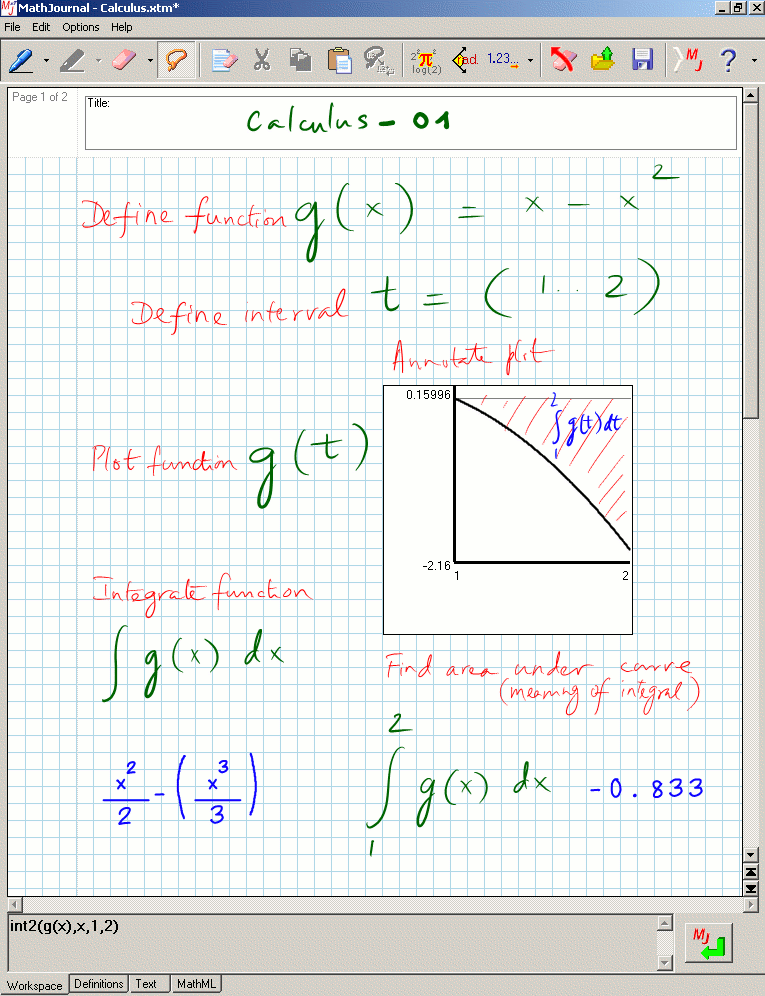
\includegraphics[width=.9\textwidth]{figures/mathjournal.png}
  \end{center}
  \caption{MathJournal}
  \label{fig:mathjournal}
\end{figure}

\subsection{Weitere}
\label{sub:mathbrush}

Die aktuelle Literatur beschreibt weitere Systeme, die Wege erforschen, interaktive Mathematik auf dem Computer durch natürliche handschriftliche Eingabe zu erleichtern. Dabei ist MathBrush \cite{Labahn:2008p10301} zu erwähnen, das ein Experimentelles Projekt ist um die handschriftliche Eingabe für Formeln in ein echtes \ac{CAS} zu ermöglichen und dann zu manipulieren. \citet{Vuong:2010p10279} stellen ein web-basiertes Handschrift-Mathematik-System vor, das eine flexible mobile Umgebung zum Lösen mathematischer Probleme bieten soll. Als Backend wird Maple \cite{maple} verwendet. Sie gehen also nach der Erkennung weiter als Programme, wie Microsoft Math und MathJournal, die eher als erweiterter Taschenrechner mit Handschrifteingabe zu sehen sind.
% Implementierung ist sogar ähnlich wie bei mir: AJAX, SVG etc.

Für beide Projekte bleiben die Probleme der eigentlichen Eingabe natürlich dieselben.

\section{Was ist so schwierig?}

Das Problem teilt sich dabei in drei Teile auf. Das erste ist die Segmentierung der mathematischen Formel, bei der einzelne Symbole isoliert werden müssen. Als zweites müssen die einzelnen Symbole richtig erkannt werden. Schließlich müssen die Symbole über ihre räumliche Position in eine logische Beziehung zueinander gebracht werden. Die in diesen Schritten gewonnenen Erkenntnisse können natürlich die Entscheidung in den jeweils anderen beeinflussen, indem man die Semantik einer Interpretation in der Erkennung mit einfließen lässt. \cite{Tapia:2007p9160} ist ein aktueller Übersichtsartikel, der die Problematik genauer beleuchtet.

Das Problem ist also sehr komplex. Entsprechend treten ständig Erkennungsfehler auf und diese zu korrigieren ist mit allen Programmen, die ich testen konnte, nicht ideal gelöst. Im Gegenteil ist der Korrekturvorgang eher langwierig und frustrierend.

\section{Suche nach Alternativen}
\label{sec:alternativen}

Die optimale Eingabemethode ist also (noch) nicht praktikabel. Um ganze Formeln zuverlässig zu erkennen haben wir noch nicht die optimalen Erkennungsalgorithmen und das optimale Benuzterinterface um mit Fehlern umzugehen gefunden. Eine Alternative ist, dem Computer nur einen Teil der Erkennung zu übertragen. Ein Beispiel hierfür ist JEquation \cite{jequation}. In diesem Programm wird dem Benutzer vorgegeben, wo der zu malen hat, damit die Struktur der Formel richtig erkannt wird. Es bleibt also die Aufgabe die einzelnen Symbole zu erkennen. Abbildung \ref{fig:jequation} zeigt dieses Benutzerinterface.

\begin{figure}
  \begin{center}
    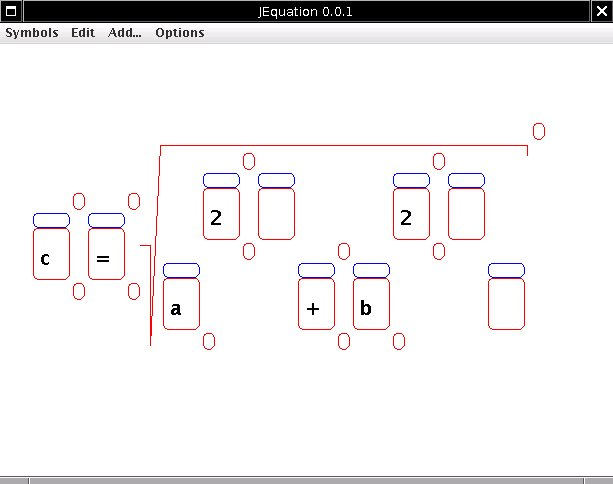
\includegraphics[width=.8\textwidth]{figures/jequation.png}
  \end{center}
  \caption{JEquation}
  \label{fig:jequation}
\end{figure}

Es gibt natürlich auch Ansätze, die ohne jede Form von Mustererkennung auskommen. Hier ist \href{http://lyx.org}{Lyx} ein Beispiel. Lyx ist ein \ac{WYSIWYM}-Editor. Er funktioniert also ähnlich wie ein \ac{WYSIWYG}-Editor wie MS-Word. Dabei arbeitet man nicht direkt mit \LaTeX-Befehlen sondern hat einen graphischen Editor in dem man jedoch die Textabschnitte semantisch auszeichnet, statt den Schriftstil manuell vorzugeben. Für Mathematische Formeln enthält Lyx einen Formeleditor, der ähnlich dem funktioniert, was aus Office-Paketen wie MS-Word bekannt ist. Um Symbole einzufügen hat man einerseits die Möglichkeit direkt \LaTeX-Befehle (mit Auto-Vervollständigung) direkt einzugeben, oder das gesuchte Symbol aus mehreren Symboltabellen auszuwählen und per Klick einzufügen. Die erste der beiden Möglichkeiten setzt natürlich wieder voraus, dass der Author den Namen des Befehls kennt. Die zweite Methode hat den Nachteil, dass die Symboltabellen schnell unübersichtlich werden, wenn sie zu umfangreich sind. Es lässt sich also nur ein kleiner Teil der verfügbaren Symbole unterbringen, ohne den Nutzen zu kompromittieren.

\section{Ein pragmatischer Ansatz} % (fold)
\label{sec:pragmatisch}

Viele Benutzer fühlen sich aber durchaus wohl damit ihre Dokumente direkt im Quelltext zu bearbeiten. Texteditoren wie Vim, Emacs etc. erfreuen sich großer Beliebtheit zum erstellen von Dokumenten \cite{latex-editor-windows, latex-editor-linux}. Ich selbst ziehe den Texteditor TextMate trotz umfangreicher Recherchen in diesem Bereich jedem spezialisierten \LaTeX-Editor vor. Die Frage ist also, wie ein pragmatisches Werkzeug aussieht, dass einem typischen Anwender die Arbeit an seinem Dokument insbesondere die Eingabe von mathematischen Formeln erleichtert ohne dessen Arbeitsweise komplett umzukrempeln.

Ein Problem, das jeder Anwender egal ob Einsteiger oder Fortgeschrittener einmal hat, ist, dass er den Befehl für ein Symbol nicht weiss. Vielleicht hat er ihn noch nie gebraucht, oder er ist ihm entfallen. Das Symbol ist auch nicht in den Symboltabellen in seinem \LaTeX-Editor (falls er nicht sowieso einen Texteditor verwendet). Also muss er ein Buch oder die "`Comprehensive \LaTeX\ Symbol List"'~\cite{Pakin:2009p2664} wälzen, um das gewünschte Symbol zu finden. Das geht bei der großen Anzahl an Symbolen~\footnote{\cite{Pakin:2009p2664} listet 4947 unterschiedliche Symbole auf.} nicht besonders schnell. Genau hier könnte ein pragmatisches Werkzeug ansetzen und auf einem Mittelweg zwischen den in \ref{sec:alternativen} vorgestellten Werkzeugen eine Lösung für dieses Problem anbieten.

Das Werkzeug müsste also eine Symbolsuche bieten, durch die sehr schnell der Befehl zum gesuchten Symbol gefunden werden kann. Der Benutzer kann sein Dokument im Editor seiner Wahl bearbeiten und im Bedarfsfall das Suchwerkzeug aufrufen, um schnell wieder an die eigentliche Arbeit, das Verfassen des Dokuments, zu gehen. Um ein solches Werkzeug wird es im Folgenden gehen.

% % section ein_pragmatischer_ansatz (end)
% 
% \section{Bemerkungen}
% 
% Auch wenn das ultimative Ziel weiterhin das in \ref{sec:optimal} skizzierte Werkzeug ist, und bei der Aufzählung der verfügbaren Software klar ist, dass viel in diese Richtung gearbeitet wird, so ist das hier beschriebene Werkzeug selbst wenn das Ziel erreicht ist nicht nutzlos. Es gibt immer Fälle in denen ... Bla.
